\documentclass[11pt,letterpaper]{article}

\usepackage[margin=2.35cm,headheight=15pt]{geometry}
\usepackage[T1]{fontenc}
\usepackage{lmodern}
\usepackage[spanish,es-nodecimaldot]{babel}
\usepackage{graphicx}
\usepackage{booktabs}
\usepackage{tabularx}
\usepackage{array}
\usepackage{xcolor}
\usepackage{fancyhdr}
\usepackage{titlesec}
\usepackage{enumitem}
\usepackage{hyperref}
\usepackage{caption}
\usepackage{float}
\usepackage{tikz}
\usetikzlibrary{arrows.meta,positioning,babel}

\definecolor{RoadGreen}{HTML}{164B3B}
\definecolor{RoadTeal}{HTML}{197A89}
\definecolor{RoadBlue}{HTML}{245A8D}
\definecolor{RoadLight}{HTML}{EDF4F0}
\definecolor{RoadGray}{HTML}{53665F}

\hypersetup{
  colorlinks=true,
  linkcolor=RoadBlue,
  urlcolor=RoadTeal,
  pdftitle={Proyecto de Sistemas Embebidos: Interfaz de alimentación},
  pdfauthor={Roderic David Munguia Calvillo}
}

\pagestyle{fancy}
\fancyhf{}
\fancyhead[L]{\small\sffamily RoadLink}
\fancyhead[R]{\small\sffamily Interfaz de alimentación}
\fancyfoot[C]{\small\sffamily\thepage}
\renewcommand{\headrulewidth}{0.4pt}
\renewcommand{\headrule}{\hbox to\headwidth{\color{RoadTeal}\leaders\hrule height \headrulewidth\hfill}}

\titleformat{\section}{\Large\bfseries\sffamily\color{RoadGreen}}{\thesection}{0.7em}{}
\titleformat{\subsection}{\large\bfseries\sffamily\color{RoadTeal}}{\thesubsection}{0.7em}{}
\titlespacing*{\section}{0pt}{2.2ex plus 0.8ex}{1.0ex}
\titlespacing*{\subsection}{0pt}{1.7ex plus 0.5ex}{0.7ex}
\setlist[itemize]{leftmargin=1.5em,itemsep=0.25em,topsep=0.35em}
\renewcommand{\arraystretch}{1.22}
\newcolumntype{Y}{>{\raggedright\arraybackslash}X}
\emergencystretch=1.5em

\begin{document}

\begin{titlepage}
  \pagecolor{RoadLight}
  \begin{center}
    \vspace*{1.0cm}
    {\sffamily\bfseries\fontsize{20}{24}\selectfont\color{RoadTeal} ROADLINK}\par
    \vspace{0.35cm}
    {\color{RoadTeal}\rule{0.82\textwidth}{2.2pt}}\par
    \vfill
    {\sffamily\bfseries\fontsize{28}{34}\selectfont\color{RoadGreen} Proyecto de Sistemas Embebidos}\par
    \vspace{0.35cm}
    {\sffamily\bfseries\fontsize{38}{44}\selectfont\color{RoadBlue} Interfaz de alimentación}\par
    \vspace{0.8cm}
    \vfill
    \begin{tabular}{>{\sffamily\bfseries}r >{\sffamily}l}
      Autor: & Roderic David Munguia Calvillo \\
      Proyecto: & RoadLink \\
      Fecha: & 29 de septiembre de 2026 \\
    \end{tabular}
    \vfill
    \begin{minipage}{0.82\textwidth}
      \centering
      \colorbox{RoadGreen}{\parbox{0.94\textwidth}{\centering\color{white}\sffamily\small
        Alimentación desde OBD-II, conversores reductores y plano de tierra}}
    \end{minipage}
    \vspace*{0.8cm}
  \end{center}
\end{titlepage}
\nopagecolor

\pagenumbering{roman}
\tableofcontents

\begin{thebibliography}{4}
\bibitem{sim800l} SIMCom, \emph{SIM800L Hardware Design},
\href{https://cn.simcom.com/product/SIM800L.html}{ficha del fabricante}.
\bibitem{a7670} SIMCom, \emph{A7670 Series Hardware Design},
\href{https://en.simcom.com/product/A7670X.html}{ficha del fabricante}.
\bibitem{esp32} Espressif Systems, \emph{ESP32-WROOM-32 Datasheet},
\href{https://documentation.espressif.com/esp32-wroom-32_datasheet_en.html}{documentación del fabricante}.
\bibitem{buck} Texas Instruments, \emph{LM2596 Step-Down Voltage Regulator
Datasheet}; referencia general del funcionamiento de un reductor ajustable,
\href{https://www.ti.com/lit/ds/symlink/lm2596.pdf}{hoja de datos}.
\end{thebibliography}

\clearpage
\pagenumbering{arabic}

\section{Introducción}

La interfaz de alimentación lleva la energía del vehículo a los circuitos de
RoadLink. La entrada se toma del conector OBD-II y se distribuye a dos
convertidores reductores de corriente continua. Uno se dedica exclusivamente al
módulo celular; el otro alimenta el ESP32 y los demás subsistemas. Esta división
se adoptó porque el módem puede exigir corriente de manera brusca al registrarse
en la red o transmitir, mientras que el controlador, la pantalla y los sensores
necesitan una tensión estable para seguir funcionando.

El presente informe describe el recorrido eléctrico visible en el prototipo y
los criterios para comprobarlo. Los consumos específicos de las placas completas
todavía deben medirse; las cifras de las hojas de datos corresponden a los
componentes, no necesariamente a las placas comerciales que los incorporan.

\section{Recorrido de la energía}

El positivo procedente de OBD-II pasa por el interruptor principal y llega a
las entradas de ambos reductores. El primero se ajusta a \textbf{4 V} para la
alimentación del SIM800L en el prototipo inicial o del A7670SA en la etapa
posterior: se utiliza \emph{un solo módem a la vez}. El segundo se ajusta a
\textbf{5 V} y abastece la placa ESP32, la pantalla TFT, el GPS, la interfaz CAN
y la demás electrónica que corresponda a esta rama. Los componentes que
internamente trabajan a 3,3 V dependen de su propio regulador o circuito de
adaptación; los 5 V no se aplican directamente a sus pines de 3,3 V.

\begin{figure}[H]
  \centering
  \begin{tikzpicture}[
    >=Latex,
    block/.style={draw=RoadTeal,fill=RoadLight,rounded corners=2pt,
      minimum height=0.95cm,text width=2.35cm,align=center,font=\small\sffamily},
    arr/.style={-{Latex[length=2mm]},thick,color=RoadBlue}
  ]
    \node[block] (obd) at (0,0) {Conector OBD-II\\alimentación del vehículo};
    \node[block] (sw) at (3.5,0) {Interruptor\\principal};
    \node[block] (b4) at (7.0,1.0) {Buck 4 V\\solo módem celular};
    \node[block] (b5) at (7.0,-1.0) {Buck 5 V\\electrónica general};
    \node[block] (sim) at (10.5,1.0) {SIM800L o A7670SA\\uno a la vez};
    \node[block] (logic) at (10.5,-1.0) {ESP32, TFT, GPS,\\CAN y periféricos};
    \draw[arr] (obd) -- (sw);
    \draw[arr] (sw.east) -- (b4.west);
    \draw[arr] (sw.east) -- (b5.west);
    \draw[arr] (b4) -- (sim);
    \draw[arr] (b5) -- (logic);
  \end{tikzpicture}
  \caption{Distribución funcional de los dos rieles de alimentación. El retorno
  de ambos se une en el plano de tierra de la PCB.}
  \label{fig:recorrido}
\end{figure}

La Figura~\ref{fig:recorrido} representa la función eléctrica, no la posición
exacta de todas las pistas. Los terminales de datos del conector OBD-II se
tratan por separado en la documentación de CAN y OBD-II.

\section{Los dos convertidores reductores}

En el montaje se emplean dos pequeñas placas \emph{buck} ajustables. Un reductor
conmutado transforma la tensión variable de entrada en una salida menor; su
potenciómetro permite fijar la tensión antes de conectar la carga. En las placas
del prototipo se distinguen el inductor, los capacitores de entrada y salida y
el ajuste. Que dos placas tengan el mismo aspecto no implica que sus salidas
puedan intercambiarse: una se reserva para 4 V y la otra para 5 V.

\begin{figure}[H]
  \centering
  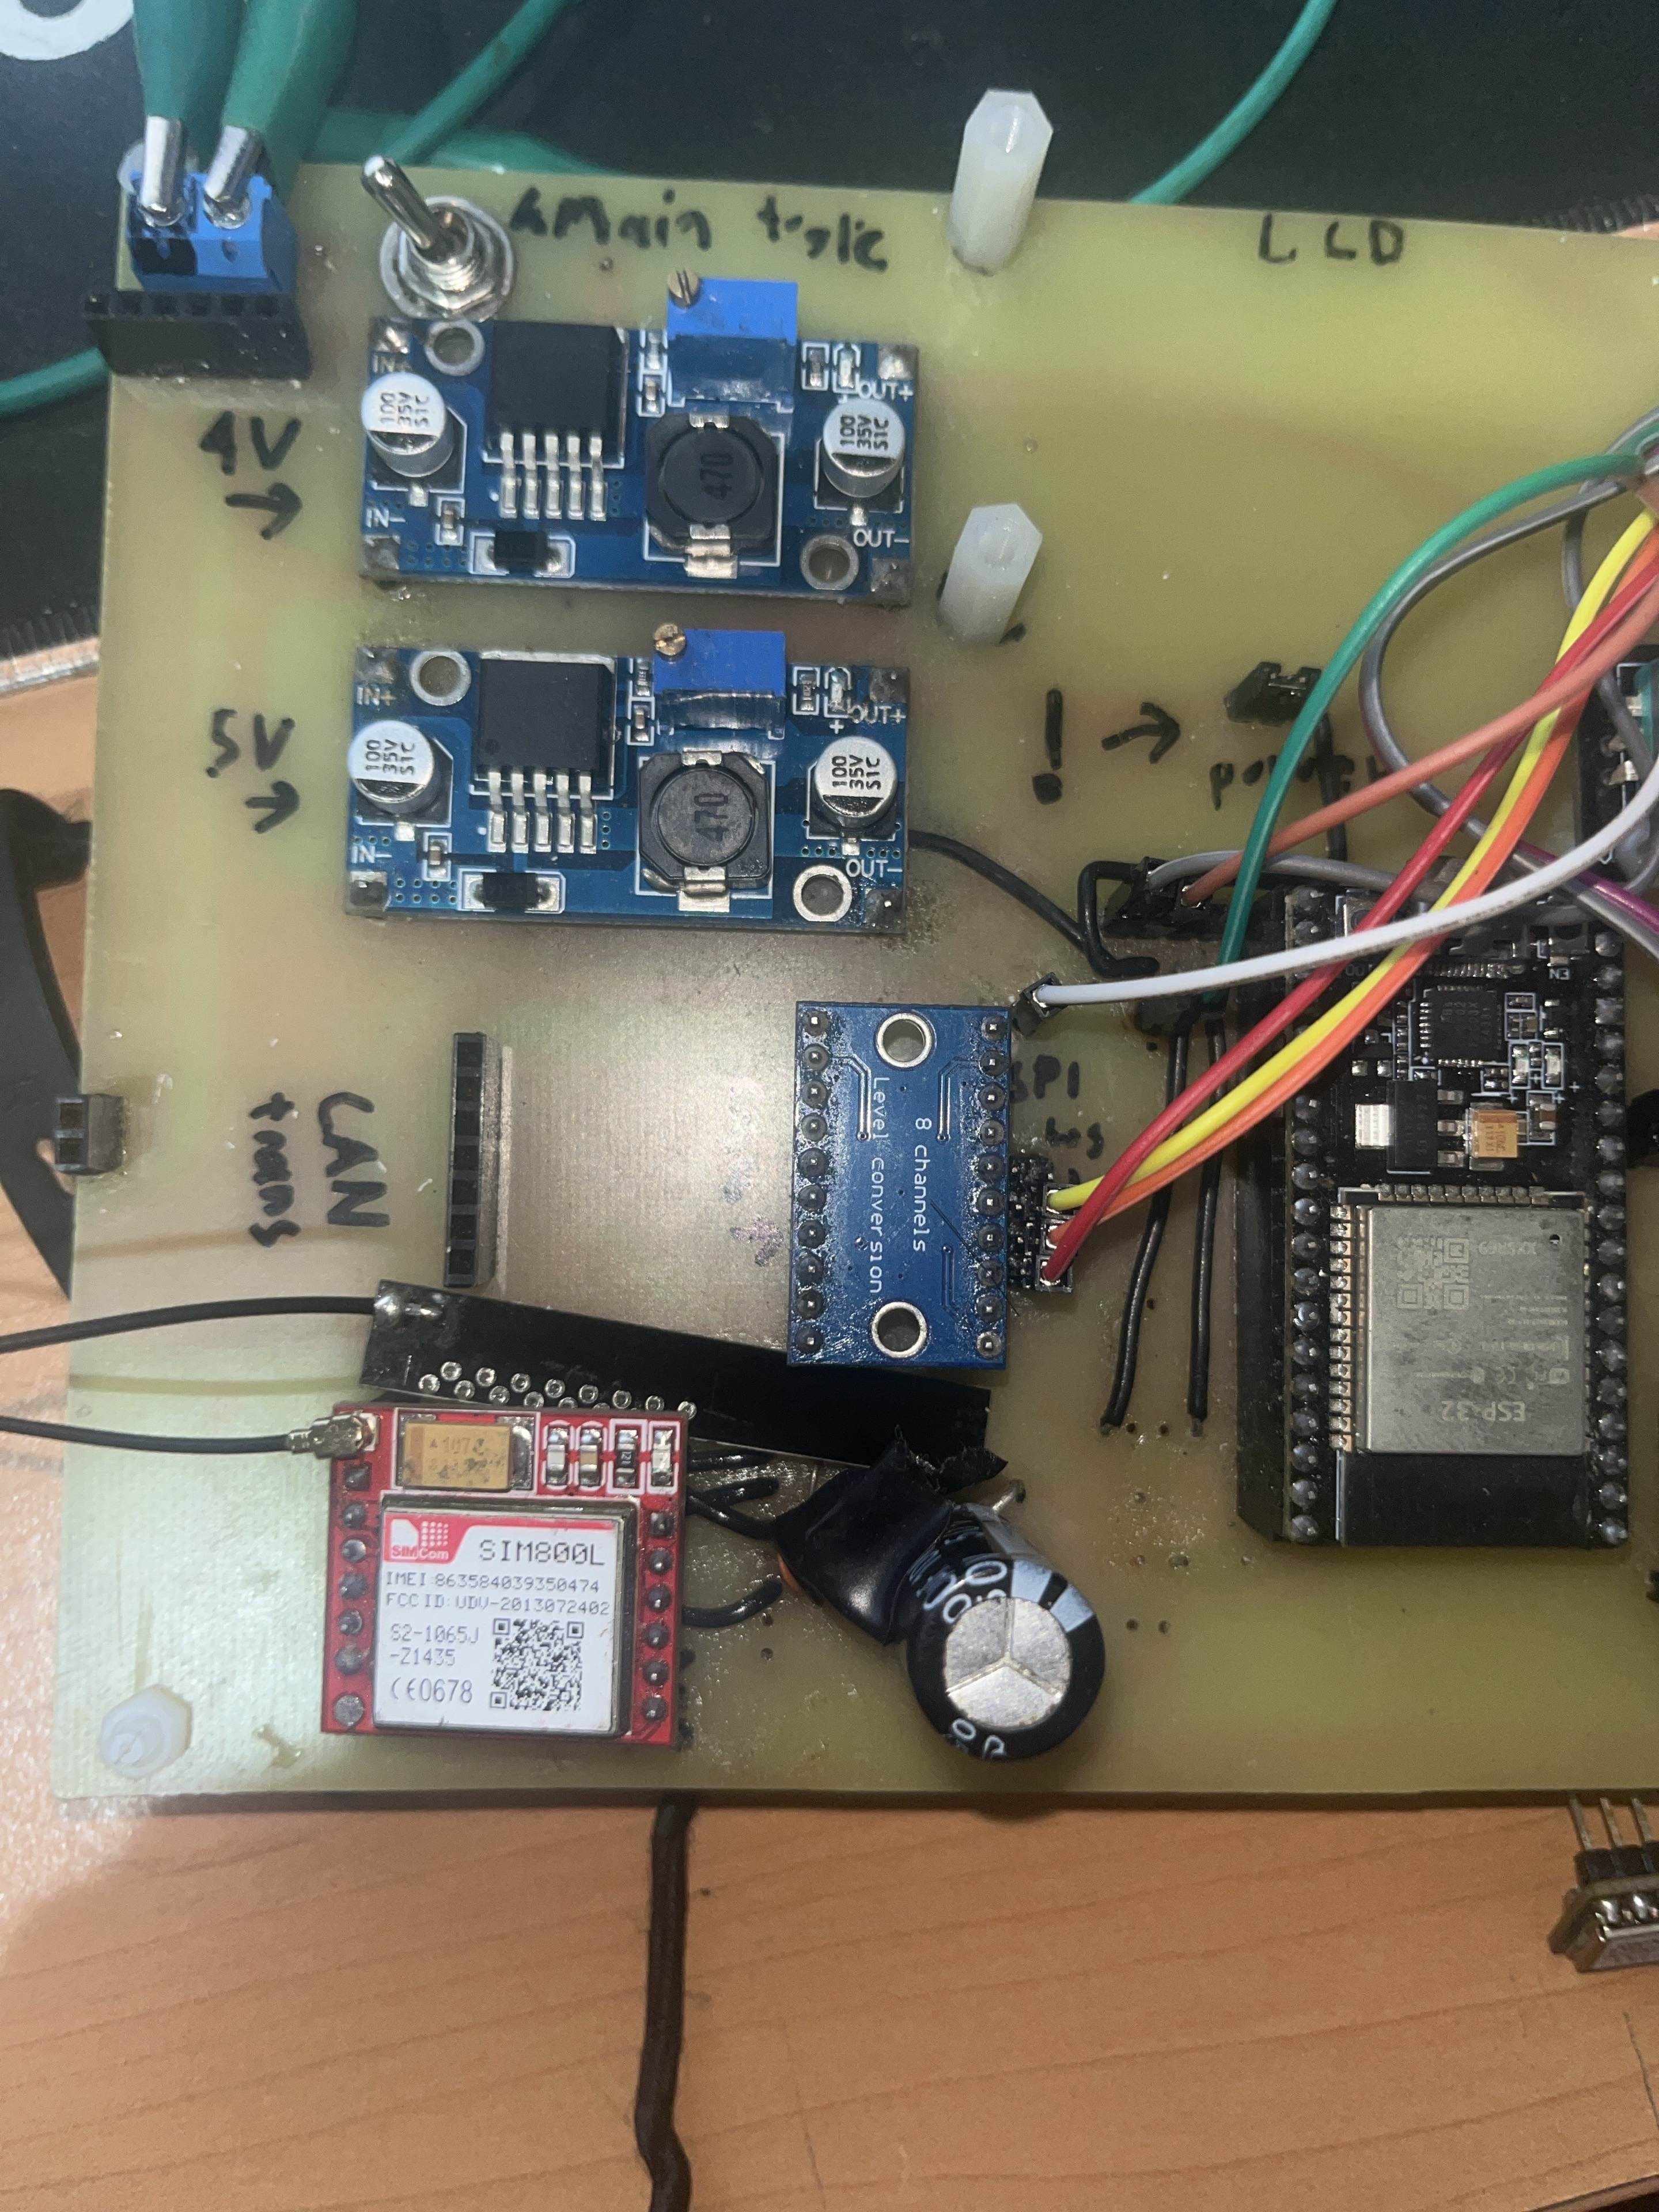
\includegraphics[width=0.57\textwidth,height=7cm,keepaspectratio]{../../recursos/imagenes/esp32-sim800l-montaje-prueba.jpg}
  \caption{Prototipo con los dos módulos reductores ajustables, la placa ESP32
  y el SIM800L. Las anotaciones de 4 V y 5 V distinguen las dos salidas.}
  \label{fig:reductores}
\end{figure}

La rama celular no toma energía del pin de 5 V ni del regulador del ESP32. Así,
un pico de corriente del módem no se suma directamente a la carga del reductor
de la lógica. Sin embargo, ambos reductores comparten la entrada del vehículo y
la referencia de tierra; no constituyen fuentes aisladas galvánicamente.

\section{Plano de tierra de cobre}

En la PCB se dejó una superficie amplia de cobre conectada a GND. Esta zona
constituye el retorno común para la entrada, los dos reductores y los módulos.
Su extensión ayuda a ofrecer una trayectoria de baja impedancia y una referencia
común para señales como UART, SPI y CAN. También evita depender únicamente de
una pista de tierra estrecha para toda la corriente del sistema.

El plano no elimina por sí solo el ruido: las ráfagas del módem todavía pueden
producir caída de tensión en conectores, cables y tramos compartidos de retorno.
Por ello interesa que la alimentación y la conexión a tierra del módem sean
cortas y de sección suficiente, y que el ESP32 mida una referencia estable en
su propia placa. La continuidad entre las tierras de ambos reductores debe
verificarse antes de conectar la comunicación UART.

\section{Carga en reposo y durante la actividad}

La demanda total depende del estado de cada subsistema. En particular, no se
debe dimensionar la rama celular usando solo la lectura de corriente en reposo:
al registrar la SIM o transmitir pueden aparecer ráfagas breves mucho mayores.
Las guías de hardware de SIMCom para estas familias describen picos de corriente
del orden de \textbf{2 A} en condiciones de transmisión; este valor es una
referencia de diseño y no una medición del montaje de RoadLink
\cite{sim800l,a7670}.

\begin{table}[H]
  \centering
  \caption{Comportamiento esperado de las cargas del prototipo.}
  \begin{tabularx}{\textwidth}{>{\bfseries\raggedright\arraybackslash}p{2.6cm} >{\raggedright\arraybackslash}p{1.8cm} Y Y}
    \toprule
    Subsistema & Rama & En espera o reposo & Actividad que eleva la demanda \\
    \midrule
    SIM800L o A7670SA & 4 V & Registrado o a la espera de enviar; el consumo depende del modo de red. & Registro, búsqueda de red y transmisión: ráfagas de corriente. \\
    ESP32 & 5 V & Ejecuta el programa y conserva las interfaces activas. & Procesamiento, comunicaciones y actualización simultánea de periféricos. \\
    Pantalla TFT & 5 V & Su retroiluminación puede seguir consumiendo aunque la imagen no cambie. & Mayor brillo y refresco de la pantalla. \\
    GPS, CAN y OBD-II & 5 V & Consumo de base de los módulos instalados. & Adquisición, recepción y transmisión de datos. \\
    \bottomrule
  \end{tabularx}
\end{table}

La placa ESP32 funciona internamente a 3,3 V, aunque el montaje la alimente
mediante la rama de 5 V; el valor final de corriente depende de la placa, del
regulador y de los periféricos conectados \cite{esp32}. Para GPS, TFT y CAN no se
asigna aquí una corriente nominal única, pues sus modelos y condiciones de uso
pueden variar. La corriente de la rama de 5 V se determina sumando mediciones de
las placas reales, incluida la retroiluminación de la pantalla.

\section{Verificación del montaje}

Antes de alimentar la PCB desde un vehículo conviene comprobar:

\begin{itemize}
  \item la polaridad y la tensión de entrada en el conector OBD-II;
  \item 4 V y 5 V en las salidas de los reductores \emph{sin carga} y después con
    las cargas conectadas;
  \item la continuidad del plano de tierra y la ausencia de cortocircuitos
    entre los dos rieles;
  \item la tensión en los terminales del módem durante el registro y la
    transmisión, cuando una caída breve podría provocar reinicios;
  \item la corriente total con el sistema inactivo y durante el uso. La toma
    OBD-II puede permanecer energizada con el vehículo apagado, de modo que el
    consumo en reposo también afecta a la batería.
\end{itemize}

El límite continuo real de cada placa \emph{buck} y su calentamiento se validan
en el montaje completo. Una cifra anunciada para el circuito integrado no
garantiza por sí sola la misma capacidad en una placa comercial con distinto
inductor, diodo, disipación y cableado \cite{buck}.

\section{Conclusiones}

La interfaz de alimentación de RoadLink parte del conector OBD-II y divide la
energía en dos salidas: 4 V exclusivos para el módem y 5 V para el controlador y
los periféricos. El amplio plano de cobre GND une los retornos y ofrece una
referencia común. La separación de rieles protege la estabilidad de la lógica
frente a las demandas rápidas del módem, siempre que la fuente de entrada, los
reductores y las conexiones soporten esas demandas.

Quedan como evidencias por registrar las tensiones y corrientes medidas en
reposo, con la pantalla encendida y durante una transmisión celular, así como
la temperatura de ambos reductores tras una operación prolongada.

\end{document}
